\documentclass[10pt,twocolumn,letterpaper]{article}
\usepackage[margin=0.8in,columnsep=0.28in]{geometry}
\usepackage[T1]{fontenc}
\usepackage{newtxtext,newtxmath}
\usepackage{microtype,amsmath,booktabs,graphicx,url,xcolor,placeins}
\usepackage[colorlinks=true,allcolors=blue!45!black]{hyperref}
\usepackage[font=small,labelfont=bf]{caption}
\setlength{\parskip}{0pt}
\setlength{\parindent}{1em}
\renewcommand{\topfraction}{0.9}
\renewcommand{\dbltopfraction}{0.9}
\renewcommand{\textfraction}{0.05}
\title{State Locality and Load Balance in Multi-LoRA Inference Pools}
\author{Spindle routing study}
\date{October 14, 2026}
\begin{document}
\raggedbottom
\maketitle
\begin{abstract}
Multi-LoRA inference pools must place adapter weights, reusable prompt state,
and request demand together. Conversation affinity preserves prefixes but can
replicate each adapter across enough engines to enlarge their working sets and
reduce effective batching. We describe an admission router that combines
measured token work with demand-sized adapter domains. Independent frontends
prefer a bounded set of replicas for each exact adapter version, preserve
observed cache matches, and escape congested placements using a work budget
expressed in engine batches. No cluster-wide coordinator lies on the custom
selection path.

We evaluate real inference on eight H200 GPUs with a hybrid 27B model,
64 saved adapter versions, and controlled general-serving and independent
single- and multi-turn RL-shaped workloads. In two order-reversed 64-version
trials, domains improve throughput over KV affinity by 59.1--62.8\%, reduce
p95 request latency by 52.3--52.7\%, and reduce GPU adapter loads by
85.5--89.1\%. These gains occur despite a 10.1--11.2 percentage-point decrease in KV
hit ratio. Warmer, smaller working sets accompany larger running batches while
requests are queued. RL-shaped replays show smaller and mixed improvements:
rollout time, individual request latency, and replay throughput can move in
different directions; a 1,024-token control regresses in window throughput and
latency. The results establish a substantial fixed-pool serving
benefit, while exposing the limits of local observations, affinity exceptions,
and replay-based claims about training throughput.

\end{abstract}

\section{Introduction}
A shared inference pool multiplexes independent fine-tuning jobs onto replicas of
one base model. Each job produces an evolving sequence of LoRA adapters and
submits batches of sampled responses. A router must place these requests while
accounting for three different kinds of state: adapter weights in host memory,
adapter weights in GPU memory, and reusable attention or recurrent state for a
particular prompt and adapter version. Spreading requests uniformly can replicate
all three. Keeping every request with its cached state can leave other replicas
idle while a hot job accumulates a queue.

The relevant unit of work is often larger than an individual HTTP request. A
single-turn reinforcement-learning rollout samples several answers for each
problem. A multi-turn rollout generates responses that become part of later
prompts. Independent jobs finish rollouts and publish new policies at different
times. Consequently, the router sees repeated, overlapping bursts rather than
synchronized cluster-wide steps. A policy that performs well on independent,
short prompts can behave differently on these workloads.

This study examines admission routing in Spindle's Modal Flash inference pool.
The engine already supports continuous batching, multiple adapters, and prefix
caching. The router neither replaces those mechanisms nor migrates running
sequences. Its task is to decide where each new sequence should execute. We
measure native KV affinity, a router that minimizes estimated outstanding work,
and an adapter-domain extension that controls preferred replication according to
outstanding adapter demand. All custom decisions are made by independent
sampling frontends using periodically refreshed observations.

Our evaluation distinguishes serving throughput from training throughput.
Inference uses real GPUs and saved, independently trained checkpoints. Recorded
optimizer/publication intervals drive the replay clients, but the evaluation
does not execute new optimization steps. The multi-turn experiments execute
causally dependent generation; synthetic tool replies control the additional
context length. These distinctions constrain the conclusions drawn from the
results.

\section{Background and Related Work}
\paragraph{Multi-adapter execution.}
Punica introduces kernels that batch computation across LoRA adapters, while
S-LoRA combines heterogeneous adapter execution with memory management for
adapter weights and KV state~\cite{punica,slora}. Those mechanisms concern the
work performed inside a serving engine. We retain the deployed engine and study
how requests are distributed among replicas. A routing gain here should not be
compared numerically with a kernel-level speedup against an engine that lacks
batched LoRA execution.

\paragraph{Adapter placement and migration.}
dLoRA jointly considers adapter execution and placement~\cite{dlora}. Its local
mechanisms choose merged or unmerged execution and protect adapters from
starvation. Its cluster mechanisms estimate queue and adapter-loading delays,
place adapters, and migrate requests with their associated state. Our work-score
baseline shares the idea of comparing dimensioned service costs. The important
system difference is that Spindle performs distributed admission decisions
through Flash, without changing execution modes or moving an active request's KV
state. We compare these design choices, not the performance of a partial dLoRA
implementation.

LoRAServe adapts placement and routing to demand and rank heterogeneity, with a
cluster orchestrator and remote adapter access over RDMA~\cite{loraserve}.
Demand-dependent placement is therefore not, by itself, a new contribution.
Our candidate instead asks how much of that benefit is obtainable from independent
frontends, shared storage, and approximate observations. This evaluation uses one
adapter rank and does not establish robustness to rank interference.

\paragraph{Distributed prefix locality.}
Preble coordinates prefix reuse and load through global and local scheduling,
including cache-eviction feedback~\cite{preble}. DualMap assigns requests to a
small candidate set and incorporates hotspot handling~\cite{dualmap}. These
systems motivate two distinct requirements: actual cache observations are more
informative than recent-use hints, and unrestricted candidate selection can
replicate state unnecessarily. Their global coordination and migration mechanisms
are not present in our router. Classical independent-balls load bounds also do
not directly apply to correlated rollout bursts with stale observations.

LMetric uses a multiplicative combination of new prefill work and batch
size~\cite{lmetric}. Its analysis identifies long, shared-prefix bursts as a
failure case: the cache advantage can continue to dominate even as a small set of
replicas becomes congested. This case is directly relevant to RL sampling. We
use that insight to motivate workload selection and explicit congestion handling.
We do not present our work-score or adapter-domain policy as LMetric, nor claim
to reproduce that paper's experimental system.

\section{System Model and Measurement}
\begin{figure*}[t]\centering
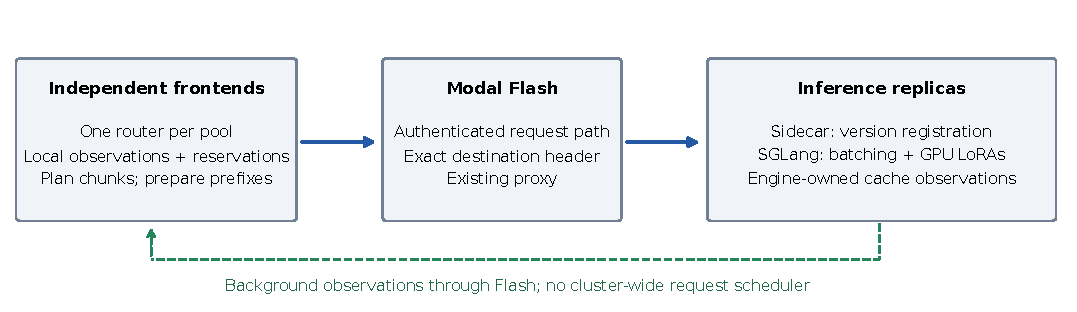
\includegraphics[width=\textwidth]{figures/architecture.pdf}
\caption{Custom request routing retains the Modal Flash transport. Each frontend
plans from its own observations and reservations. The engine remains responsible
for exact cache matching and adapter execution. Observation traffic is shared
information, not distributed admission control.}\label{fig:architecture}
\end{figure*}
\subsection{Request path and ownership}
A sampling frontend receives a group of generation requests, identifies the
immutable adapter version, and selects a destination for each sequence. Requests
still traverse the authenticated Modal Flash endpoint. Custom routes use the
exact-upstream header; competing native-affinity headers are removed. The
sidecar resolves the adapter snapshot, registers it with SGLang when necessary,
and forwards generation to the engine. Exact version checks are independent of
cache and load estimates.

Each frontend owns one router per inference pool, shared by the pool's adapters.
There is no coordinator that serializes all sampling requests. The router's
selection method is synchronous and does not acquire an asynchronous lock.
Frontends periodically discover membership and poll replicas concurrently. A
fresh selection reads local state. Startup and expired observations can coalesce
behind one bounded refresh; failed discovery falls back to native Flash.

The engine owns cache truth. A CPU-only observer snapshots reusable cache
boundaries, outstanding request identifiers, remaining token work, and CPU/GPU
adapter sets approximately once per second. A bounded background writer handles
file I/O. The sidecar combines that snapshot with requests that have arrived but
are not yet visible to the scheduler. Frontends discard observations whose reported
engine age exceeds three seconds. This includes the individual probe's round-trip
time, but excludes time subsequently spent waiting for another probe in the same
refresh; it is not a strict three-second end-to-end freshness bound.
Membership is rediscovered approximately every five
seconds. These are eventual observations, not a global admission protocol.

\subsection{Cache identity and correctness}
The cache key includes the exact adapter identity and token prefix. Updating an
adapter invalidates routing credit for the old version even when the prompt is
unchanged. Hashes are computed at 64-token boundaries; the final prompt token is
never credited because its logits must be evaluated. A hash receives credit only
if the engine advertises that boundary as reusable. An observation replaces the
previous set, so evicted entries do not persist as positive hints indefinitely.
Each snapshot advertises at most 8,192 prefix boundaries. Entries omitted by
that limit receive no routing credit even if the engine could reuse them.

The deployed model is hybrid: a reusable boundary requires both the attention
state and the corresponding recurrent-state checkpoint. Merely observing a radix
path is insufficient. Unsupported cache configurations receive no credit. Hash
collisions or stale positive observations could affect placement quality; they
cannot cause the engine to reuse an invalid cache entry, because the engine
performs its own match using its original token and adapter identity.

\subsection{Costs and their limits}
We measure aggregate prefill rate $r_p$, aggregate decode rate $r_d$, effective
running capacity $C$, GPU adapter-loading delay $t_g$, and registration delay
$t_c$ on the deployed model and hardware. These quantities have physical units;
there is no arbitrary coefficient adding a dimensionless hit ratio to a queue
length. Nevertheless, the model is approximate. Prefill cost depends on context
and batch shape, output limits overestimate early-EOS decoding, and host elapsed
load time is not an isolated GPU-transfer measurement.

In the pinned engine, registration runs synchronously on the scheduler path.
The router therefore accounts for registration as additional work rather than
assuming it overlaps all queued inference. Volume and operating-system caches
make registration latency state dependent. We do not claim that unregistering an
adapter forces a network-cold checkpoint read.

\section{Routing Policies}
\subsection{Native KV affinity}
The main baseline sends a stable affinity key through Flash. It preserves the
relationship between a conversation or sampling group and a replica as long as
the infrastructure preserves that mapping. It does not consult our engine cache
observations or adapter-working-set state. We measure its actual placement and
balance; affinity is not treated as a proof that every request will reach the
same host under failures or membership changes.

Conversation affinity can also spread one adapter across many engines even
without a hot conversation. Under an idealized independent, uniform mapping,
$m$ conversation keys visit an expected
$N[1-(1-1/N)^m]$ of $N$ replicas. With four keys and eight replicas, that is
3.31 replicas per adapter. A catalog that fits once in aggregate GPU adapter
memory can therefore exceed that capacity several times over when each key is
placed independently. This occupancy calculation motivates controlling adapter
replication separately from preserving an individual conversation's prefix.
It is not an assertion about Flash's mapping implementation.

\subsection{Estimated-work routing}
For incoming prompt length $P$, output limit $D$, and replica $i$, let $H_i$ be
the longest advertised reusable prefix. Its estimated per-sequence work is
\begin{equation}
  w_i = (P-H_i)/r_p + D/r_d.
\end{equation}
The replica backlog $B_i$ sums observed remaining prefill and decode work,
plus local reservations not yet represented in the observed request-ID set.
Adapter setup is charged once per distinct pending cold adapter: $t_g$ when
absent from GPU memory and $t_c$ when absent from registered host state. Let
$A_i$ be the corresponding setup cost of the incoming adapter if it is not
already resident or pending. For a placement chunk of $g\le C$ siblings,
\begin{equation}
  S_i = B_i + A_i + g w_i.\label{eq:work}
\end{equation}
The work router chooses the smallest $S_i$. Numerical ties preserve the previous
prefix destination, then use deterministic rendezvous ordering.

A group larger than $C$ is split into chunks. Siblings in a chunk retain the
chosen host while it remains eligible; retries can select again. Each sequence
reserves its local estimated work before sending the HTTP request and releases
that reservation on success, failure, or cancellation. Observed request IDs
prevent double counting. The unsent remainder of a group is not a cluster-wide
reservation, and different frontends can still select the same replica before
observing one another's decisions.

Equation~\ref{eq:work} estimates drain work, not the completion time of a
continuous-batching simulation. It can overestimate queued prefill when the
engine has not yet matched that request's cache. It also does not predict repeated
adapter evictions caused by interleaving a working set larger than GPU capacity.
These limitations motivate the replication experiment rather than an additional
unmeasured eviction coefficient.
The engine also constrains admission by the union of adapters already decoding
and those entering prefill. With overlap loading disabled, a request introducing
an adapter beyond the eight-adapter batch limit is skipped, even if sequence
slots remain~\cite{sglang-admission}. A scalar transfer charge alone does not
model that compatibility constraint.

\subsection{Demand-sized adapter domains}
Unrestricted work minimization can spread a cold adapter to every replica before
any frontend observes the resulting queue. Subsequent requests then compete with
more adapter versions at each engine. Charging one transfer per adapter does not
capture the repeated eviction and reload of that adapter. We address this
failure with a preferred replica set, rather than another additive penalty.

\paragraph{Preferred placement.}
Let $\mathcal A$ be the observed catalog of exact adapter versions and $N$ the
replica count. Each frontend independently orders $\mathcal A$ and assigns a
primary replica to each entry. For adapter $a$, replicas are ordered by
rendezvous hashing. The primary is the first replica minimizing
$\lfloor n_i/S\rfloor$, where $n_i$ is the number of primaries already assigned
to replica $i$ and $S$ is its adapter-slot budget. The remaining replicas follow
the adapter's rendezvous order. This deterministic computation is cached until
the catalog or topology changes.

For a common catalog and topology with $|\mathcal A|\le NS$, no replica has more
than $S$ preferred primaries: while any replica has fewer than $S$, its quotient
is zero and a replica already at $S$ cannot receive another primary. This is a
property of the preferred map, not an invariant on GPU contents. Replication,
different frontend observations, base-model health probes, and cache-preserving
exceptions can all increase the working set beyond the preferred budget.

\paragraph{Demand-dependent replication.}
Let $q_a$ be outstanding requests for exact adapter $a$, including the incoming
chunk and local reservations not represented in the observed request IDs. The
preferred domain is the first
\begin{equation}
 k_a=\min\{n,\max\{1,\lceil q_a/C\rceil\}\},
\end{equation}
where $n$ is the currently eligible replica count; the domain uses the first
$k_a$ entries of the retained placement order and dispatch filters out ineligible
entries. A cold, low-demand adapter initially uses one
replica; each additional engine-sized batch of demand permits another. A hot
adapter can eventually use the whole pool. A replica with an actual reusable
prefix remains a candidate even outside the preferred domain. Thus the policy
does not discard useful KV state solely to enforce an adapter map.

\paragraph{Congestion escape.}
For a newly planned chunk, first compute the work score on every eligible
replica. Let $S_* = \min_i S_i$, and let
$\Delta=C\max_i w_i$ be a budget expressed as one engine batch of charged
per-sequence work. Retain domain or cache-bearing replicas only when
$S_i\le S_*+\Delta$. Choose the smallest score among them; if none remain,
choose the global minimum. Consequently, a new placement cannot sacrifice more
than $\Delta$ of \emph{estimated} drain work to locality in that local view.
This statement is not a bound on request latency: observations are stale,
continuous batching is approximate, and siblings retain a previously planned
host. Choosing one batch as the tolerance is a design heuristic, not an optimum
derived from a queueing model.

\paragraph{Stable observation handling.}
Rebuilding every primary map after a single missing observation can move
unrelated adapters. The stable variant retains topology and catalog entries for
the router's ten-second stale horizon. Eligibility for dispatch remains stricter:
an engine observation with reported age above three seconds cannot receive an explicit
selection. A temporarily missing primary therefore spills its own requests
without immediately remapping every other primary. Frontends do not agree on a
membership epoch; persistent failure and catalog churn can still cause movement.

\begin{table}[t]\small
\begin{tabular}{p{0.95\columnwidth}}
\toprule
\textbf{Domain placement for a new chunk}\rule{0pt}{2.5ex}\\
1. Read eligible observations; add unobserved local reservations to their work.\\
2. Find each replica's longest exact-version token-prefix match $H_i$.\\
3. Reuse or rebuild the slot-budgeted primary map; expand this adapter's domain to $k_a$ replicas.\\
4. Compute $S_i$ for every eligible replica and its minimum $S_*$.\\
5. Among domain members or cache-bearing replicas with $S_i\le S_*+\Delta$, choose minimum $S_i$. If empty, choose the global minimum.\\
6. Retain the chunk destination. Reserve each sibling before its HTTP dispatch; release it when that attempt finishes.\\
\bottomrule
\end{tabular}
\caption{Placement procedure. All state and decisions in this procedure belong
to one frontend. Missing fresh observations cause native-Flash fallback.
An already planned chunk normally reuses its eligible destination.}
\label{tab:algorithm}
\end{table}

\paragraph{Preparing a sampling cohort.}
For sibling responses to a prompt of length $P$, define the largest eligible
boundary $b=64\lfloor(P-1)/64\rfloor$. Before dispatching the siblings, the
prototype plans their destinations and locally reserves their work. On each
selected replica lacking that boundary, it generates one auxiliary token from
the first $b$ input tokens. That token is discarded. The actual sibling prompts
and sampling parameters are unchanged. All preparation time and auxiliary work
are included in the evaluation.

Preparation changes the charged prefill work for a chunk of $g$ siblings to
\begin{equation}
 U_i(g)=\frac{\max(0,b-H_i)+g[P-\max(H_i,b)]}{r_p}.
\end{equation}
The score becomes $B_i+A_i+U_i(g)+gD/r_d$, and each sibling reserves
$U_i(g)/g+D/r_d$. This amortized value also replaces $w_i$ in the congestion
escape budget. This accounts for one shared prefill and the unavoidable
suffix of every sample. It is used only in the preparation variants. Planning
without preparation would underestimate cold work. Preparation does not pin the
cached boundary: eviction before a sibling executes can invalidate this cost
estimate. Single-sequence requests,
including later dialogue turns, use the original score.

Prefix preparation itself is not a new serving primitive. The pinned SGLang
tokenizer manager already warms a prompt before expanding native parallel
sampling~\cite{sglang}. Spindle's separate HTTP samples do not take that path.
Our experiment applies the primitive across selected pool destinations and
tests the same preparation with native KV affinity. This control is necessary
to isolate a routing contribution.

\paragraph{Concurrency and cost.}
Only the frontend's own event loop serializes its short selection calculation.
There is no request-time distributed lock or coordinator RPC. Engine polling is
off the ordinary selection path. Prefix hashes are computed once in preparation
and once in dispatch, then reused by siblings within each phase.
Selection scans eligible replicas, their advertised cache boundaries, and
unobserved local reservations. A retained chunk normally checks one destination.
The observation traffic still grows as $O(FN)$ for $F$ frontends and $N$
replicas. Moving coordination off the request path does not remove that scaling
cost or guarantee globally balanced decisions.


\section{Experimental Methodology}
\paragraph{Hardware and engine.}
All new GPU experiments use the same eight H200 replicas in Modal's us-west
region, with one GPU, eight CPU cores, and 64\,GiB of host memory per replica.
The base model is \texttt{Qwen/Qwen3.8-27B}, loaded as
\texttt{Qwen3\_5ForConditionalGeneration}; its hybrid attention/recurrent cache
is relevant to the matching procedure. Tensor, data, and pipeline parallelism
are each one. Context capacity is 16,384 tokens and the static memory fraction
is 0.8. The engine is SGLang v0.5.17 with the pinned Modal fork and routing
instrumentation (Appendix~\ref{sec:reproduce}). The cached model download records
revision \texttt{1d4bf0f2ff6012fd82039f2fa52739d0dd7c60c0}.
Its text configuration declares BF16; the engine's weight and KV dtype options
are \texttt{auto}. A live settings audit records FA3 attention, FlashInfer
sampling, CSGMV LoRA execution, CUDA graphs enabled, 8,192-token chunked prefill,
16,384 maximum prefill tokens, and page size one. The model configuration and
its SHA-256 are included in the artifact.

The engine uses longest-prefix-match scheduling, eight GPU adapter slots,
256 host adapter slots, and no overlapping LoRA loading. Adapters have rank 32
and update the query, key, value, output, gate, up, and down projections.
Although the configuration requests 128 running sequences, the deployed engine
reports an effective capacity of \textbf{36 per replica}, or 288 for the pool.
All capacity comparisons use that observed value. The Flash target concurrency
is 64 and the minimum and maximum replica counts are both eight. These are
fixed-pool experiments; they do not evaluate an autoscaling controller.

\paragraph{Calibration.}
A separate pre-experiment run measures aggregate rates on each replica and uses
their median: $r_p=8{,}706$ input tokens/s, $r_d=1{,}065$ output tokens/s,
$t_g=0.0672$\,s, and $t_c=1.871$\,s. These values remain fixed for the
comparisons. Registration measures exposed elapsed delay, including shared
storage and software overhead; it is not a guaranteed network-cold transfer.
The transfer estimate is the median backend-latency difference between paired
cold-GPU and hot-GPU requests with the same 128-token prompt and cache match.
Eight independent 8,192-token prompts estimate prefill rate; a warmed batch of
36 requests generating 512 tokens estimates decode rate. Separately, engine
load counters record host elapsed loading calls without CUDA synchronization.
Neither those summed counters nor the calibration differences are added
directly to a claimed wall-time saving.

These measurements also constrain what the score can plausibly optimize. One
GPU adapter load corresponds to approximately 585 uncached input tokens at the
measured prefill rate; one registration corresponds to approximately 16,287.
Reusing a 7,168-token prefix is therefore more valuable in this model than
avoiding one GPU load, but less valuable than avoiding one registration. These
are comparisons of calibrated work terms, not predictions of isolated request
latency. Repeated eviction and different batch shapes can change the realized
cost.

\paragraph{Checkpoints and clients.}
Sixteen independently trained DAPO math clients supply real checkpoint
identities and recorded update/publication intervals of approximately 34--96\,s.
Each delay is that source client's measured second update, from training start
to publication, reused as a constant in later replay rounds.
The RL-shaped replays use versions 4 and 7. A general-serving stress test uses
versions 4, 7, 10, and 13 from these jobs: 64 different checkpoint files,
verified by distinct SHA-256 digests. This represents 64 adapter versions, not
64 independent training jobs. Each checkpoint is approximately 319\,MB.

RL-shaped experiments use eight distinct CPU frontend containers (two CPU cores
and 8\,GiB each), two independent clients per frontend, and one router shared by
those two clients. A training client's requests originate from one frontend;
these GPU experiments do not test simultaneous same-adapter arrivals from many
frontends.
The dedicated benchmark frontends invoke the shared \texttt{sample\_task}
execution path directly. They bypass the public control-plane command queue;
reported request latency begins at frontend preparation, not at SDK submission.
Each client starts after a 0.5\,s incremental offset. After its initial rollout,
it overlaps the next rollout with its own recorded update delay. There are no
cross-client round barriers. At the next eligible round it switches to the
specified saved checkpoint. We validate independent progress from rollout
timestamps, not from launch staggering alone. Optimizers do not execute during
these replays; results concern inference under a training-shaped arrival process.

\paragraph{Controlled prompts and generations.}
\begin{table*}[t]\centering\small
\begin{tabular}{lrrrrrr}\toprule
Workload & Clients & Versions used & Sequence ceiling & Samples/group & Input/output tokens & Generations\\\midrule
Warmed reuse & 16 & 16 & 1,024 & 8 & 8,192 / 256 & 3,072\\
Version turnover & 16 & 32 & 1,088 & 8, 64, 128 & 8,192 / 256 & 4,352\\
Three-turn dialogue & 16 & 32 & 512 & $8\rightarrow1$ & 8,192--9,216 / 256 & 4,608\\
General serving & 16 & 64 & 512 & 1 & 8,192 / 512 & 2,048\\
Longer decode & 16 & $\le32$ & 1,088 & 8, 64, 128 & 8,192 / 512 or 1,024 & Variable\\
\bottomrule\end{tabular}
\caption{HTTP/2 workload definitions. ``Clients'' counts independent checkpoint
sources; general serving has eight streams per exact version. The sequence
ceiling is potential logical concurrency, not a claim that all streams are
simultaneously in an engine. All workloads share eight GPUs and 288 effective
running slots. Dialogue continuations use single-sequence requests. Longer
decode admits new rollouts for 300 seconds (512 outputs) or 180 seconds
(1,024 outputs), then drains already submitted work.}
\label{tab:workloads}\end{table*}
To control cost, long prompts contain 7,168 tokens shared by a client's problem
across rounds and a 1,024-token round-specific suffix. Tokens are sampled
deterministically from the vocabulary occurring in that client's DAPO prompts.
Thus the lengths and sharing structure are controlled, but the resulting long
text is synthetic. Output lengths are fixed with \texttt{ignore\_eos=True};
the principal RL comparisons generate 256 tokens per request. This is not an
evaluation of answer quality or the natural EOS-length distribution.

The warmed workload gives each of 16 clients eight problem groups and eight
samples per group: 1,024 potential concurrent sequences. The initial HTTP/1
phase uses four rounds (4,096 generations); the subsequent HTTP/2 comparisons
use three (3,072 generations), permitting repeated trials within the allocation.
Three serial one-token warmup requests per problem
establish reusable prefixes before timing. The version is fixed, while suffixes
change across rounds.

The turnover workload preserves the same total demand for 15 clients but
changes its concentration. Clients 1--7 each submit one group of 64 siblings;
client 0 submits one group of 128; clients 8--15 retain eight groups of eight.
The ceiling is 1,088 concurrent sequences and the four rounds contain 4,352
generations. Versions 4 and 7 serve two rounds each. Only version 4 is registered
initially; version 7 incurs real first-use registration during measurement.
This shape stresses a few popular affinity keys while other clients continue
independently.

The dialogue workload uses four groups of eight initial samples per client,
three dependent generation turns, and three rollout rounds. Its ceiling is
512 active sequences and it contains 4,608 generations. Each continuation
appends the actual preceding 256-token response and a 256-token synthetic tool
reply, producing input lengths 8,192, 8,704, and 9,216. The first group finishes
before its branches continue; later branches progress independently. Adapter
identity is fixed within a trajectory and changes between rollout rounds.

The final general-serving workload uses all 64 saved versions, eight independent
streams per version, four prefix groups per version, and four requests per
stream. It therefore has 512 concurrent streams and 2,048 requests. Inputs are
8,192 tokens with 7,168-token shared prefixes; outputs are 512 tokens. Each
stream waits for its previous request, but the returned text is not appended in
this workload. Eight independent router objects run in one eight-core CPU
container; this tests independent router state, not eight-process overhead.
Each router shard has its own HTTP/2 generation client, and a separate client
collects observations. These eight generation connections permit the intended
concurrency despite the client's per-connection stream cap.
All versions are registered before timing. The separate stress pilot doubles
the streams and uses three requests per stream (1,024 concurrency, 3,072 total).

RL sampling uses temperature 1 and deterministic per-request seeds derived from
4242, the round, group, and sibling index. General serving uses temperature 0
and sampling seed $12026+100\times\text{stream index}+\text{turn}$.
Prompts, checkpoint identities, and requested output limits are
identical across policies within each trial.

The longer-decode controls retain the version-turnover shape and run independent
loops for a 300\,s rollout-admission window with 512-token outputs and a 180\,s
window with 1,024-token outputs. The latter window is shortened before launch
to fit the unchanged GPU deadline, equally for both policies.
Already submitted rollouts finish after that window. We report completions in
the interval from 60\,s to each window's end separately from total replay time
and drain time.
Because faster clients start subsequent rollouts earlier, these are closed-loop
rate measurements with policy-dependent request totals, not fixed-work makespan
comparisons. A 100-round guard is not reached in the measured window.

\paragraph{Comparisons and reset.}
The main controls are native KV affinity (KV), KV with cohort preparation
(KV+P), and stable adapter domains with preparation (Domains+P). The turnover
experiment also includes unrestricted estimated-work routing with preparation
(Work+P). General serving additionally tests the default SDK path with no
caller-supplied cache-affinity key; its ordinary per-request session header
remains present. Thus ``default'' does not mean removing every routing header.
The initial comparison orders KV before KV+P before Domains+P;
repeated comparisons reverse the latter pair. Every final trial unregisters the
entire previous adapter catalog, registers the prescribed initial versions,
materializes the base-model health-probe slot, and flushes prefix state.
Warmup, registration, and frontend startup are outside the measurement interval.
On-demand registration of new versions and cohort preparation are inside it.

\paragraph{Transport amendment.}
The initial stress trials use HTTP/1 with a 240\,s timeout; the subsequent
four-policy turnover and warmed trials increase it to 600\,s. Warmed trials
still encounter roughly 360\,s read failures after requests disappear from
engine observations. We preserve these runs and stop the unfinished HTTP/1
suite. A separate phase enables HTTP/2 for every arm, validates greedy cohort
equivalence again, and asserts that every successful physical generation
attempt records HTTP/2 trace events. The server advertises 1,024 concurrent
streams. We do not compare throughput across transport phases as a routing
effect, and do not claim that HTTP/2 alone establishes the root cause of the
HTTP/1 failures. The allocation deadline is extended by 45 minutes to run this
controlled phase; the GPU count remains eight.

The first general-serving HTTP/2 attempt exposed an additional client-side
limit. HTTPcore 1.0.9 permits only 100 streams on one connection, despite the
server's higher limit. That attempt shared one connection between generation
and observation, reached only 82 observed active requests, and had observation
gaps up to 180\,s. We preserve its completed default arm as a diagnostic and
restart every general-serving policy with eight generation connections and a
separate observer. The RL replays already have eight independent frontend
clients. Corrected general-serving arms must observe at least 288 active pool
admissions; this validates pressure at the pool boundary, not GPU utilization.
The RL frontends retain the same 100-stream-per-connection limit under every
policy. Their logical concurrency ceilings can therefore exceed actual HTTP
concurrency. In the first trials, measured peak pool admissions are 461--480
for warmed reuse, 542--600 for turnover, and 375--400 for dialogue, all above
the pool's effective running capacity. We report both configured demand and
observed pressure rather than equating them.

\paragraph{Metrics and validation.}
Useful throughput counts only requested output tokens. Request latency begins
before cohort preparation and ends when that individual sample completes;
rollout latency ends after the client's entire batch or dialogue finishes.
Replay makespan includes the recorded update intervals, including the final
overlapped interval. We therefore report rollout latency alongside replay
throughput rather than interpreting all elapsed-time changes as engine capacity.

KV hit ratio is reused prompt tokens divided by requested prompt tokens.
We also account separately for auxiliary seed prefill, which can raise the
visible hit ratio without eliminating the initial computation. Hot-LoRA ratio
is the fraction of engine admissions finding the adapter GPU-resident; it
includes auxiliary seeds and physical retry admissions. Adapter load and
eviction counts come from engine counters, not router predictions. Replica load
is measured at two-second intervals; busy-balance statistics require at least
288 active pool requests. They are sampled observations, not continuous traces.

Every completed arm verifies exact start/end adapter versions, output and
log-probability lengths, finite log probabilities, unique request identities,
destination consistency, and zero final sidecar inputs. Native final queue
counts are zero except where a cached subsecond observation predates that
replica's last successful response; such cases require no retries and are
reported without changing the raw counts. Later arms poll for settled native
zeros after freezing the timer. The cohort control separately
checks that greedy outputs agree before and after preparation on all eight
replicas. Greedy token equality does not establish identical floating-point
log probabilities or training-quality equivalence. Retries, incomplete arms,
observation gaps, and exploratory trials are retained and identified explicitly.

\section{Evaluation}
\subsection{Controlled HTTP/2 comparisons}
\begin{table*}[t]\centering\small
\begin{tabular}{llrrrrrrr}\toprule
Workload / trial & Policy & Replay (s) & Output tok/s & Mean (s) & p95 (s) & Rollout (s) & KV hit & Retries\\\midrule
Warmed reuse 1 & KV+P & 289.1 & 2721 & 30.1 & 56.4 & 46.7 & 0.940 & 0 \\
Warmed reuse 1 & Domains+P & 275.9 & 2851 & 29.9 & 58.0 & 43.5 & 0.953 & 0 \\
Warmed reuse 2 & KV+P & 289.8 & 2714 & 33.3 & 61.0 & 48.2 & 0.930 & 0 \\
Warmed reuse 2 & Domains+P & 284.7 & 2762 & 31.0 & 61.7 & 43.2 & 0.963 & 0 \\
Version turnover 1 & KV+P & 355.9 & 3130 & 39.2 & 81.6 & 51.8 & 0.955 & 0 \\
Version turnover 1 & Domains+P & 350.8 & 3176 & 28.8 & 61.3 & 37.7 & 0.970 & 0 \\
Version turnover 2 & KV+P & 354.8 & 3140 & 39.3 & 81.0 & 49.6 & 0.956 & 0 \\
Version turnover 2 & Domains+P & 365.0 & 3052 & 31.0 & 58.9 & 39.0 & 0.965 & 0 \\
Dialogue 1 & KV+P & 376.8 & 3130 & 18.5 & 49.8 & 90.5 & 0.951 & 0 \\
Dialogue 1 & Domains+P & 316.9 & 3722 & 21.4 & 43.8 & 78.8 & 0.905 & 0 \\
Dialogue 2 & KV+P & 362.1 & 3257 & 18.7 & 50.4 & 87.5 & 0.950 & 0 \\
Dialogue 2 & Domains+P & 295.7 & 3989 & 20.5 & 38.3 & 79.6 & 0.916 & 0 \\
64 versions 1 & KV & 440.5 & 2381 & 60.1 & 237.6 & -- & 0.654 & 0 \\
64 versions 1 & Domains & 270.6 & 3875 & 53.9 & 113.4 & -- & 0.542 & 0 \\
64 versions 1 & Default & 544.2 & 1927 & 111.3 & 200.7 & -- & 0.053 & 0 \\
64 versions 2 & KV & 427.1 & 2455 & 61.1 & 245.2 & -- & 0.649 & 0 \\
64 versions 2 & Domains & 268.5 & 3906 & 53.8 & 116.0 & -- & 0.548 & 0 \\
Long 512 & KV+P & 415.9 & 4491 & 71.3 & 155.5 & 99.0 & 0.970 & 0 \\
Long 512 & Domains+P & 393.4 & 5414 & 62.2 & 137.5 & 81.3 & 0.956 & 0 \\
Long 1,024 & KV+P & 335.0 & 5674 & 106.0 & 200.9 & 138.2 & 0.971 & 0 \\
Long 1,024 & Domains+P & 261.6 & 6011 & 113.8 & 217.9 & 150.8 & 0.952 & 0 \\
\bottomrule\end{tabular}
\caption{Completed HTTP/2 comparisons, reported separately by trial. All times include any cohort preparation. Replay throughput includes recorded update waits for RL workloads; rollout latency excludes those waits. Trial 2 reverses policy order. No confidence interval is inferred from individual requests.}\label{tab:primary}
\end{table*}

Table~\ref{tab:primary} reports each completed trial separately. The time-series
and latency distributions use the first trial, while the repeat reverses policy
order. The paired ranges below describe these executions, rather than confidence
intervals inferred from individual requests.
The primary comparisons comprise 58,368 logical requests across 17 arms,
including the single default-policy control. All finish without retries; every
arm exceeds 288 observed active pool inputs, and every RL arm exhibits overlap
between different clients' rollout rounds.

\paragraph{Working-set pressure with 64 versions.}
Across the two order-reversed trials, Domains improves useful throughput by
59.1--62.8\%, lowers mean request latency by 10.4--11.9\%, and lowers p95 by
52.3--52.7\% relative to KV (Figure~\ref{fig:general-summary}). GPU loads fall
85.5--89.1\%. Each arm completes the same 2,048 requests without retries.
The repeat runs Domains before KV; the conclusion is not specific to which
policy runs first.

In the first corrected general-serving trial, Domains increases throughput
from KV affinity's 2,381 to 3,875 output tokens/s (62.8\%). Mean request latency
falls from 60.1 to 53.9\,s (10.4\%), and p95 falls from 237.6 to 113.4\,s
(52.3\%). Makespan falls from 440.5 to 270.6\,s. Both arms complete the same
2,048 requests with no retries and reach 512 active requests. Default routing
achieves 1,927 tokens/s, so KV affinity is already a substantially stronger
baseline than the default path.

GPU adapter loads fall from 1,168 to 169 (85.5\%) and evictions from 1,160 to
161. First-prefill hot-adapter admissions rise from 984 of 2,048 (48.0\%) to
1,864 (91.0\%). This does not come from higher prefix reuse: KV hit ratio falls
from .654 to .542, increasing uncached input by 32.3\%. The result demonstrates
a case where maximizing prefix hits is the wrong pool objective.

The aggregate KV ratio includes initially cold requests. In the first trial,
KV affinity's ratios by stream request index are 9.5\%, 77.6\%, 87.2\%, and
87.3\%. Only 7,168 of 8,192 input tokens are shared, so the last two indices
approach the workload's 87.5\% reusable fraction. The 65.4\% aggregate is not
evidence that all later affinity requests miss their prefixes. Domains' later
indices achieve 70.8\%, 72.1\%, and 72.6\%, exposing a real locality sacrifice.

Across the complete trial, an adapter version visits 3.28 replicas on average
under KV, close to the idealized four-key occupancy calculation, versus 1.41
under Domains. A prefix group visits 1.00 versus 1.11 replicas. Thus the router
primarily co-locates different conversations using the same adapter while
allowing some individual prefixes to move. Default routing visits 7.83 replicas
per adapter and 5.16 per prefix group. These are whole-trial destination counts,
distinct from simultaneous residency or active working-set measurements.

During busy observations, the mean active adapter working set per replica falls
from 22.9 to 9.3; the fraction of replica observations exceeding eight active
adapters falls from 98.7\% to 57.3\%. The mean engine-reported running count when
requests are queued rises from 16.3 to 27.5. Both policies keep every replica
nonempty during the sampled busy intervals. Thus the difference is not simply
eliminating entirely idle hosts. Smaller adapter working sets and larger running
batches accompany the throughput gain, despite additional prefill.

These observations are consistent with improved batch compatibility under the
eight-adapter admission limit. The pinned scheduler explicitly skips requests
whose adapter cannot join the running set~\cite{sglang-admission}. We do not
trace every such rejection, so the measurements do not isolate its contribution
from prefill scheduling and queue placement. Summed host elapsed loading time
falls from 86.24 to 11.01\,s;
it is not a decomposition of the 169.9\,s makespan reduction. The domain policy
still exceeds eight active adapters in some observations, as permitted by its
cache-preserving and congestion-escape rules.

The repeat also preserves the mechanism measurements. Mean busy adapter working
sets are 23.5 for KV and 8.5 for Domains; running counts while queued are 16.1
and 28.3. GPU loads are 1,234 versus 135, and hot-adapter admission ratios are
44.9\% versus 93.8\%. KV reuse falls from 64.9\% to 54.8\%. These observations
reinforce the distinction between optimizing a cache-hit metric and improving
pool completion time.

\begin{figure*}[t]\centering
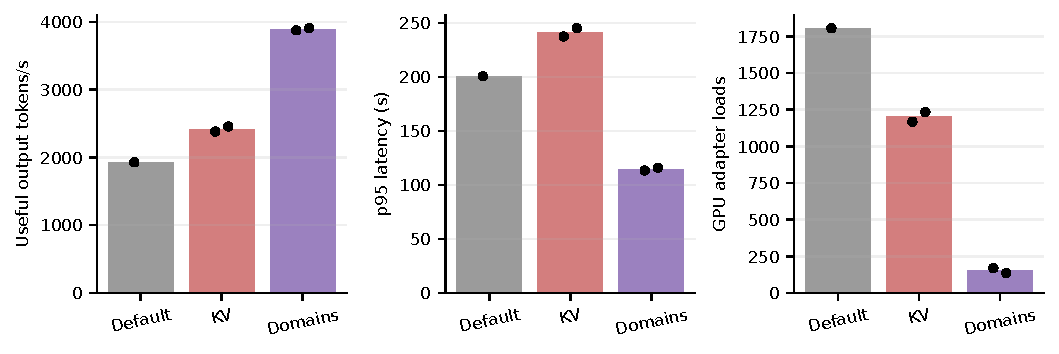
\includegraphics[width=\textwidth]{figures/general-serving.pdf}
\caption{General serving with 64 versions. Points show individual trials; bars
show their arithmetic mean, not a fitted expectation. KV and Domains have two
order-reversed trials; Default has one. All use the corrected eight-connection
HTTP/2 topology and identical requested work.}
\label{fig:general-summary}\end{figure*}

\begin{figure*}[t]\centering
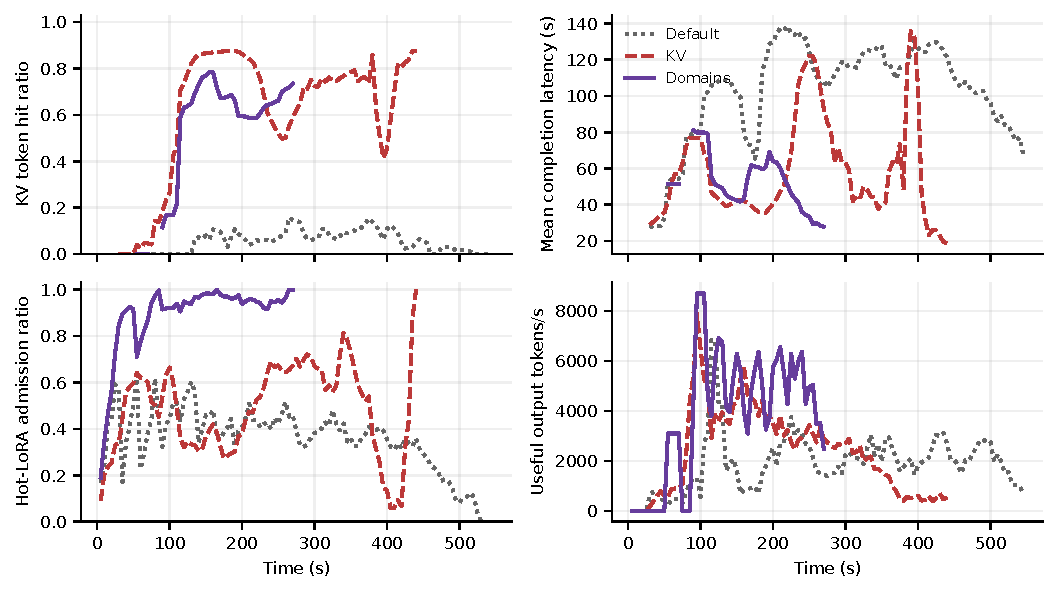
\includegraphics[width=\textwidth]{figures/general-time-series.pdf}
\caption{First corrected 64-version serving trial: 512 independent streams,
8,192-token inputs, and 512-token outputs. Domains sustains more hot-adapter
admissions while accepting fewer KV hits. The same completion-window and
counter-difference definitions as Figure~\ref{fig:timeseries} apply.}
\label{fig:general}\end{figure*}

\paragraph{Warmed reuse.}
Across the two order-reversed trials, Domains+P reduces GPU adapter loads by
43.6--52.0\% and improves replay throughput by 1.8--4.8\%. Mean rollout latency
falls 6.8--10.4\%, while eleven of sixteen clients improve in each trial.
The p95 request latency nevertheless rises 1.2--2.7\% in both trials.
Avoiding adapter movement is repeatable here, but the end-to-end throughput
benefit is much smaller than in the 64-version workload.

The requested-token KV ratio rises in both trials. Its relationship to actual
prefill work is less consistent: seed-inclusive uncached input rises from
13.4\% to 14.5\% of logical input in the first trial, but falls from 14.9\% to
13.6\% in the repeat. Each arm issues 384 seeds. Counting those seeds' uncached
input is necessary to interpret the apparent cache improvement.

\paragraph{Skew and new versions.}
Across both trials, mean request latency falls 21.0--26.5\%, p95 falls
24.9--27.2\%, and mean rollout time falls 21.4--27.2\%. Replay throughput
changes by $-2.8$\% to $+1.5$\%, providing no repeatable throughput improvement.
GPU loads increase 32.9--36.1\%; thirteen to fifteen clients have faster mean
rollouts. Load balancing helps most clients finish their batches sooner, but
the fixed update delays and slowest client still determine replay makespan.

In the first HTTP/2 turnover trial, Domains+P reduces mean request latency from
39.24 to 28.84\,s (26.5\%), p95 from 81.63 to 61.27\,s (24.9\%), and mean
rollout time from 51.84 to 37.72\,s (27.2\%). Replay throughput increases only
1.5\%, from 3,130 to 3,176 tokens/s. GPU loads increase from 72 to 98 and
registrations from 51 to 59: the latency improvement comes with more replication,
unlike the 64-version working-set result.

Fifteen of sixteen clients have lower mean rollout time. The client with 128
siblings improves from 71.2 to 50.0\,s; the seven clients with 64-sibling groups
average 41.9 versus 29.9\,s; and the eight clients with eight groups of eight
average 58.1 versus 43.1\,s. Thus the aggregate improvement is not confined to
the largest group. It still does not establish per-client fairness: one client
regresses, and the warmed and dialogue trials improve only eleven and ten
clients respectively.

The repeat's critical path is observable directly. Under KV+P, client 14's
59.1\,s initial rollout and three 96.2\,s update intervals finish at 354.6\,s.
Under Domains+P, client 15 becomes the last client: its initial rollout takes
68.7\,s versus 33.3\,s under KV+P, followed by three 96.2\,s intervals, finishing
at 364.8\,s. Its later rollouts are all shorter than the update delay. Improving
their mean duration therefore cannot recover the initial critical-path loss.

\paragraph{Dependent dialogue.}
Both trials improve replay throughput (18.9--22.5\%), mean rollout time
(9.0--12.9\%), and p95 request latency (12.1--24.1\%) while worsening mean
request latency (9.5--15.6\%). Ten clients improve in the first trial and eleven
in the repeat. The mean-versus-tail tradeoff is therefore present in both
policy orders.

The first dialogue trial raises replay throughput by 18.9\%, reduces mean
rollout latency by 12.9\%, and reduces p95 request latency by 12.1\%. Mean
request latency nevertheless rises 15.6\%. Per-turn measurements show that
Domains+P's later turns reuse less state: KV hit ratios are .883 and .885,
versus KV+P's .947 and .951. The seed-inclusive uncached-input fraction rises
from 7.6\% to 12.4\%.

The apparent tension between rollout and request latency is visible directly
in the trajectories. Mean time from rollout start to a trajectory's completion
increases from 58.1 to 66.3\,s. However, a finished trajectory's mean wait for
the rest of its client's rollout falls from 32.4 to 12.5\,s. Thus average full
rollout time decreases from 90.5 to 78.8\,s even though individual trajectories
finish later on average. This is a reduction in completion-time dispersion,
not evidence that every generation runs faster.
The repeat has the same pattern: mean trajectory completion rises from 59.1
to 64.6\,s, while its wait for the remaining rollout falls from 28.4 to 15.0\,s.

\begin{figure}[t]\centering
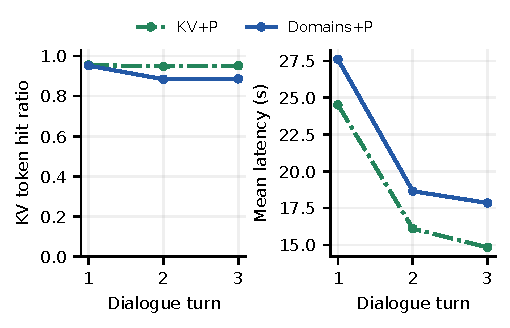
\includegraphics[width=\columnwidth]{figures/dialogue-turns.pdf}
\caption{First HTTP/2 dialogue trial. Only the first turn uses cohort preparation.
Later turns expose a cache-locality cost under Domains+P. The lower full-rollout
latency does not imply lower mean latency at each turn.}\label{fig:turns}
\end{figure}

\begin{figure*}[t]\centering
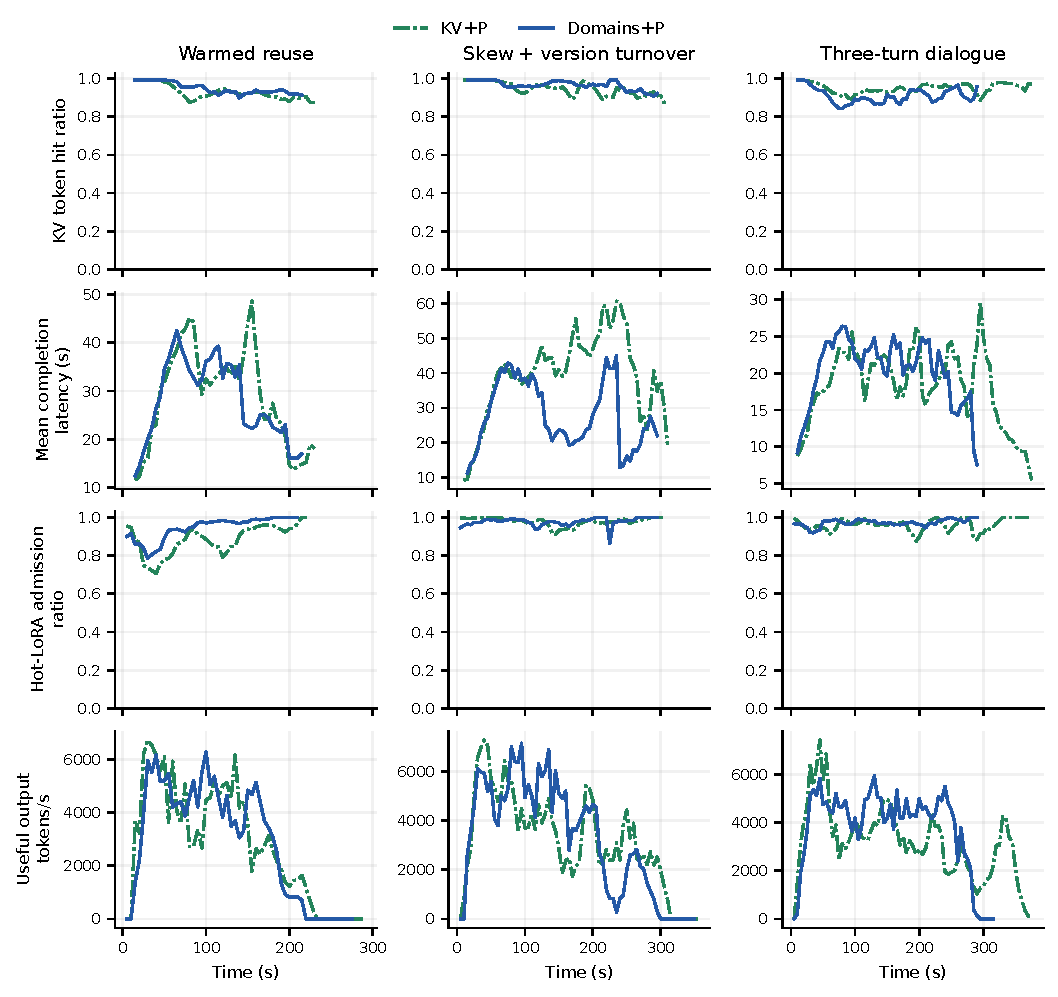
\includegraphics[width=\textwidth]{figures/time-series.pdf}
\caption{First HTTP/2 trial of each RL-shaped workload. Curves use 20-second
trailing windows sampled every five seconds. KV ratio and mean latency use
completed logical requests; hot-LoRA ratio uses interpolated engine admission
counter differences, including seeds. Useful throughput excludes seed outputs.
Windows with no relevant completions or admissions have gaps.}
\label{fig:timeseries}\end{figure*}

\begin{figure*}[t]\centering
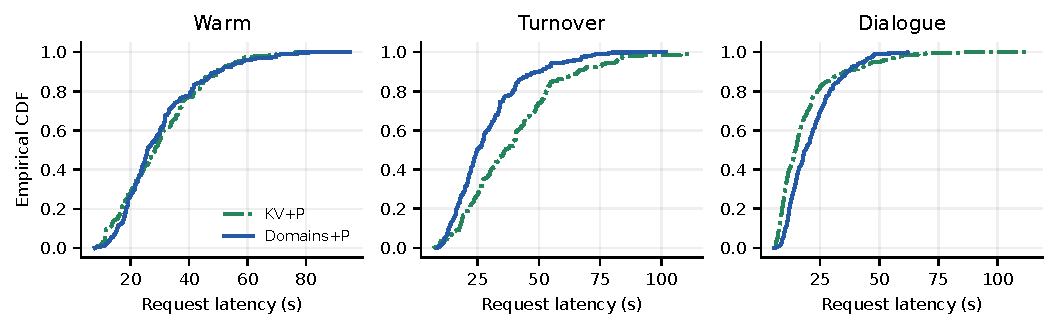
\includegraphics[width=\textwidth]{figures/request-cdf.pdf}
\caption{Individual-request latency distributions in the first HTTP/2 trials.
Each curve includes every completed logical request and any preparation time.
The samples are dependent; these CDFs are descriptive, not independent
replications.}\label{fig:cdf}\end{figure*}

\subsection{Longer generation under independent loops}
\begin{table*}[t]\centering\small\setlength{\tabcolsep}{4pt}
\begin{tabular}{llrrrrr}\toprule
Output tokens & Policy & Requests & Window completions & Window tok/s & Window mean (s) & Loads / 1k\\\midrule
512 & KV+P & 3648 & 2389 & 5097 & 71.2 & 16.4 \\
512 & Domains+P & 4160 & 2887 & 6159 & 66.5 & 23.8 \\
1,024 & KV+P & 1856 & 1068 & 9114 & 97.2 & 2.7 \\
1,024 & Domains+P & 1536 & 889 & 7586 & 106.0 & 21.5 \\
\bottomrule\end{tabular}
\caption{Longer-output controls. Window metrics use completions from 60 seconds to the arrival-window end: 300 seconds for 512-token outputs and 180 seconds for 1,024-token outputs. Admitted work drains afterward. Total work depends on policy, so loads are normalized by logical requests. Each output length has one trial.}\label{tab:long}
\end{table*}

The longer-output controls retain skewed groups and independent publication
delays. Unlike the fixed-round comparisons, clients admit new rollouts until
the same wall-clock cutoff, then drain submitted work. Faster progress changes
the number of requests and checkpoint versions encountered. Window throughput
therefore measures this closed-loop workload, not a fixed-work speedup or an
estimate of stationary engine capacity. Window latency also describes the
requests that complete in that interval, rather than all arrivals.

With 512-token outputs, Domains+P completes 2,887 requests during seconds
60--300 versus KV+P's 2,389, raising useful window throughput from 5,097 to
6,159 tokens/s (20.8\%). Across the full replay, it completes 4,160 versus
3,648 requests and achieves 5,414 versus 4,491 tokens/s (20.6\%). Mean request
latency falls from 71.31 to 62.17\,s (12.8\%), p95 from 155.49 to 137.54\,s
(11.5\%), and mean rollout time from 98.97 to 81.30\,s (17.9\%). Both arms
finish without retries. Fourteen KV+P clients and fifteen Domains+P clients
reach the second checkpoint, yielding 30 and 31 versions respectively.

The mechanism differs from the 64-version result. Busy observations with an
idle replica fall from 59.6\% to 28.1\%, while active-load variation falls from
.770 to .593. GPU loads increase from 16.4 to 23.8 per thousand logical
requests, and the seed-inclusive uncached-input fraction rises from 7.1\% to
10.5\%. The router spends more on replicated state to serve more overlapping
work. There is still substantial imbalance; these observations do not show
that every replica is saturated whenever the pool has a queue.

The 1,024-token control exposes a regression. During seconds 60--180,
Domains+P completes 889 requests versus 1,068 for KV+P: window throughput
falls from 9,114 to 7,586 tokens/s (16.8\%). Across the full replay, mean
request latency rises from 105.97 to 113.81\,s (7.4\%), p95 from 200.93 to
217.86\,s (8.4\%), and mean rollout time from 138.16 to 150.75\,s (9.1\%).
Both arms finish without retries. Busy observations with an idle replica rise
from 24.3\% to 38.5\%, and active-load variation rises from .507 to .632.
GPU loads rise from 2.7 to 21.5 per thousand logical requests; seed-inclusive
uncached input rises from 5.7\% to 9.3\%.

Full-replay throughput alone would conceal this result: it rises from 5,674
to 6,011 tokens/s (5.9\%), but Domains+P admits only 1,536 requests versus
1,856 and has a shorter drain. The fixed-window and latency measurements do
not support an improvement for this control. Only one client in each arm
reaches the next version, so it is primarily a longer-decode check, not a
broad turnover test. Each longer-output pair has one trial; the evaluation
neither attributes this regression to a single score term nor establishes
robustness across output lengths. The fixed calibration and one-batch escape
budget require further evaluation when decoding dominates.

\subsection{Why the initial policies were insufficient}
We first evaluated 512 requests from 32 adapter versions, 256 concurrent streams,
4,096-token prompts, and 128-token outputs. This pilot did not saturate the
pool's 288 running slots. Table~\ref{tab:pilot} exposes a failure of optimizing
one locality metric: the first domain policy reduced GPU adapter loads from
165 to 54, but still finished 3.7\% slower than KV affinity. Unrestricted
estimated-work routing dispersed reusable prefixes and was slower still.
These are exploratory trials used to refine the design, not independent
validation runs.

\begin{table}[t]
\centering\small
\begin{tabular}{lrrrr}
\toprule
Policy & Time (s) & KV hit & Hot LoRA & Loads\\
\midrule
KV & 42.2 & .414 & .586 & 165\\
Work & 50.6 & .017 & .426 & 316\\
Basic domains & 43.8 & .368 & .885 & 54\\
\bottomrule
\end{tabular}
\caption{Exploratory 32-adapter pilot. Lower adapter traffic alone did not
improve completion time.}\label{tab:pilot}
\end{table}

The placement map also matters when the catalog approaches aggregate slot
capacity. On the actual eight-replica topology, hashing 16 model identities and
co-locating their four versions assigned between zero and 16 preferred adapters
to each host. The excess above eight slots totaled 12 adapters. Hashing the 64
exact versions independently still left ten excess assignments. The
slot-budgeted primary map removes this particular preferred-placement
imbalance. It does not prevent later demand-driven replication from exceeding
the slot budget.

\subsection{Separating preparation from routing}
A second pilot used 16 clients, two groups of 16 siblings per client, one
rollout, 8,192-token inputs, and 128-token outputs. Preparing the shared boundary
reduced KV affinity's mean latency from 15.49 to 9.68\,s and raised useful
throughput from 2,363 to 3,559 tokens/s. Domains+P achieved 9.96\,s and 3,415
tokens/s: it did not improve on the stronger baseline. Its GPU loads were lower
(14 versus 27), yet that advantage did not determine completion time.

This pilot retained the earlier 64-entry host catalog, although only 16 versions
were used during the measured burst. The final-trial reset removes that
experiment-order dependency. We retain the pilot to explain the control and
design decisions, not as a final claim about the revised reset procedure.

\subsection{Version turnover: separating three effects}
The initial HTTP/1 turnover trial completes all four arms without a retry.
Table~\ref{tab:turnover-ablation} separates prefix preparation, load-aware
placement, and adapter domains. Relative to KV, adding preparation reduces mean
request latency by 12.6\% and increases replay throughput by 22.0\%. Its visible
KV hit ratio rises from .842 to .967, but the uncached-input fraction including
seed work falls only from 15.8\% to 8.4\%. The distinction prevents auxiliary
prefill from being mistaken for free cache reuse.

Relative to KV+P, Domains+P reduces mean request latency by 27.8\%, p95 latency
by 28.1\%, and mean rollout latency by 32.3\%. Busy observations with at least one
idle replica fall from 53.1\% to 2.0\%; the mean replica-load coefficient of
variation falls from .765 to .408. These observations support the intended
mechanism: a few congested affinity destinations no longer determine most
clients' rollout time. GPU adapter loads nevertheless increase from 66 to 88,
and seed-inclusive uncached input increases from 8.4\% to 9.7\%. The improvement
comes with additional state replication.

\begin{table*}[t]\centering\small
\begin{tabular}{lrrrrrrrr}\toprule
Policy & Output tok/s & Mean request (s) & p95 (s) & Mean rollout (s) & KV hit & Loads & Registers & Busy idle\\\midrule
KV & 2,738 & 37.44 & 72.15 & 57.74 & .842 & 66 & 51 & 65.8\%\\
KV+P & 3,341 & 32.72 & 69.08 & 47.06 & .967 & 66 & 51 & 53.1\%\\
Domains+P & 3,137 & 23.63 & 49.65 & 31.84 & .971 & 88 & 57 & 2.0\%\\
Work+P & 3,059 & 23.43 & 51.31 & 30.30 & .977 & 144 & 83 & 5.3\%\\
\bottomrule\end{tabular}
\caption{Initial version-turnover ablation: 4,352 requests per arm, 8,192 input
and 256 output tokens, eight H200 replicas, HTTP/1, no retries. Busy idle is the
fraction of sampled observations with at least 288 active requests and an idle
replica. This single trial is separate from the HTTP/2 comparisons.}
\label{tab:turnover-ablation}\end{table*}

\begin{figure*}[t]\centering
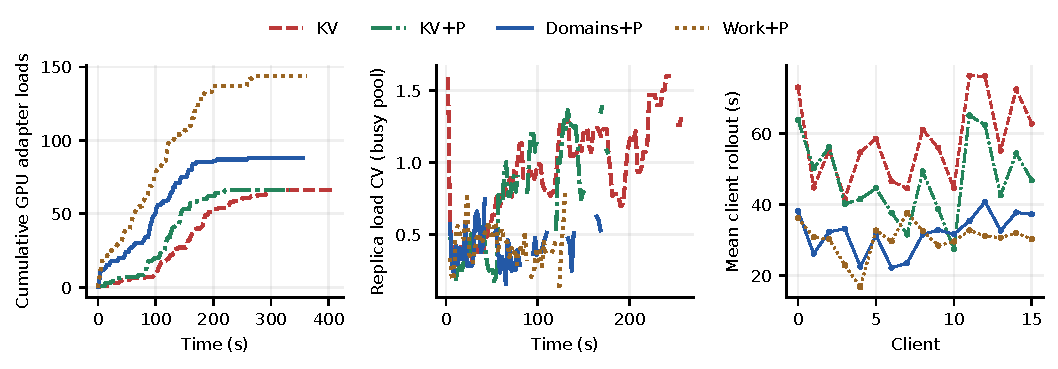
\includegraphics[width=\textwidth]{figures/turnover-mechanisms.pdf}
\caption{Initial turnover ablation. Left: cumulative GPU adapter loads. Middle:
replica-load variation when the pool has at least 288 active requests. Gaps omit
less-loaded periods. Right: each independent client's mean rollout time.
Load-aware placement improves balance; domain restriction reduces adapter
movement relative to unrestricted work routing.}\label{fig:mechanisms}
\end{figure*}

\paragraph{Why replay throughput can still decrease.}
Despite lower average latencies, Domains+P takes 355.1\,s versus KV+P's
333.5\,s, reducing replay throughput by 6.1\%. Client 15's initial rollout
takes 58.8\,s under Domains+P versus 33.5\,s under KV+P. Its later rollouts are
faster under Domains+P, but three approximately 96\,s overlapping update
intervals preserve the initial delay on the replay's critical path. The experiment
therefore demonstrates an average-latency improvement, not a training-throughput
improvement. A scheduler optimizing total work does not directly optimize each
independent training loop's completion time.

\paragraph{What the adapter domains contribute.}
Work+P has a similar mean request latency (23.43\,s versus 23.63\,s), while
Domains+P reduces GPU loads by 38.9\% (144 to 88) and registration calls by
31.3\% (83 to 57). Summed host elapsed loading time falls from 9.68 to
6.01\,s, not an additive 3.67\,s wall-clock saving. The evidence attributes much
of the latency improvement to load-aware placement and a separate reduction in
state movement to domains. It does not establish that minimizing loads alone
maximizes throughput.

\paragraph{Cache observation and preparation audit.}
Before this trial, all 72 problem groups in every arm have a reported reusable
7,168-token prefix. Missing initial cache observations therefore do not explain
the baseline comparison. Preparation also does not guarantee permanent reuse.
KV+P has 976 sibling requests with less than the prepared 8,128-token match;
all execute on their seed's replica, and 832 retain exactly the 7,168-token
prefix. Domains+P has 758 such requests, 730 on the seed's replica. Most observed
losses cannot be explained by routing to a different host. Cache eviction and
the hybrid engine's reusable-boundary behavior remain relevant after placement.

\subsection{Routing overhead}
The initial turnover run measures a 136\,$\mu$s p95 domain-selection duration
and a 1.48\,ms p95 engine snapshot duration. The mean serialized routing-state
size is approximately 8.1\,KB per replica, excluding the additional counters
collected by the benchmark observer. These measurements exclude network polling
from the synchronous selection duration; they do not imply zero control-plane
cost.

An isolated CPU benchmark uses 64 catalog entries, 36 observed requests per
replica, 128 local reservations, 8,192-token prompts, 200 warmup calls, and
1,000 measured selections. On an Intel Xeon Platinum 8375C, domain selection for
single requests has p95 costs of 150, 449, and 1,713\,$\mu$s at 8, 32, and 128
replicas. Groups of eight amortize the mean cost to 28, 68, and 252\,$\mu$s per
sibling; their p95 still includes new chunk planning. Prefix hashing separately
has a 174\,$\mu$s median in this environment. These are CPU cost measurements,
not distributed scalability experiments.

For 64 adapters, rebuilding the preferred map costs 89, 236, and
747\,$\mu$s at p95 for the same replica counts when the topology's hash orders
are retained; rebuilding those orders raises the figures to 213, 710, and
2,864\,$\mu$s. The cached map avoids that work on ordinary selections. Polling
still scales with frontend count times replica count.

\subsection{Transport-affected stress results}
The HTTP/1 64-version stress pilot uses 1,024 streams and 3,072 generations.
KV takes 533.8\,s with 202 retries; the intermediate balanced-domain policy
takes 410.0\,s with 109 retries. The apparent throughput improvement is 30.2\%,
while mean request latency increases from 84.9 to 86.8\,s. This result is
retained as a stress observation, not a clean estimate of the final policy's
routing benefit. The prototype and the retry workload both differ.

The initial warmed HTTP/1 KV and KV+P arms take 551.3 and 574.9\,s with one
and three retries respectively. In one traced failure, the request disappears
from engine observations approximately 293\,s before its HTTP read fails;
increasing the client timeout to 600\,s does not remove the roughly 360\,s
failure. These observations motivate the separate transport phase, not removal
of failed attempts from the metric denominator. The unfinished domain arm is
canceled and is not reported as a completed trial.

The single-client HTTP/2 diagnostic completes 2,048 default-policy requests in
719.5\,s, with no retries but only 1.6\% KV hits and 2,354 GPU loads. Its mean
request latency is 157.4\,s, while mean backend latency is 24.4\,s. Only nine
complete pool observations return during the run. The verified 100-stream
client cap and shared observer connection invalidate a pool-saturation claim
for this configuration. The corrected general-serving comparison changes the
client topology for every policy and is reported separately.

\FloatBarrier
\section{Discussion and Limitations}
\paragraph{Local estimates are not distributed admission control.}
An independent frontend cannot see another frontend's reservations before the
next observation. Several frontends can therefore choose the same apparently
idle replica, and a domain can grow later than the actual arrival burst.
Deterministic primary maps reduce unnecessary replication but can also correlate
those decisions. This design offers no global queue bound, no per-adapter
starvation guarantee, and no theorem of throughput optimality. Obtaining such
properties would require an admission protocol, migration, or explicit engine
scheduling support beyond this prototype.

The preferred map also counts registered versions that currently have no demand.
Long-running training can accumulate a large inactive catalog even when only a
few latest versions are sampled. The evaluated catalog contains at most four
versions per job and 64 versions overall. Demand-filtered catalog retention or
version garbage collection would require an additional policy; the present
results do not establish behavior under indefinite publication history.

The cache exception has another explicit limit: if every replica advertises
some reusable prefix for an adapter, every replica passes the locality filter.
The work score still compares the remaining prefill, but domain restriction no
longer limits that adapter's replication. A common system prefix across many
otherwise different prompts could produce this condition. Our controlled
problem prefixes are distinct, so the experiments do not resolve this case.

For example, consider eight frontends with identical empty observations, each
submitting 36 requests for the same uncached adapter before a refresh. Each
frontend sees one batch of demand and selects the same primary. Executing this
case against the actual router on CPU assigns all 288 requests to one replica.
This is a deterministic counterexample, not a GPU performance measurement. The
local score bound does not prevent this correlated-arrival case. A batched,
replica-local admission protocol could address it without a cluster-wide request
coordinator, but it is not implemented or evaluated here.

\paragraph{Autoscaling remains a separate control problem.}
Flash scales on request concurrency, whereas the router compares estimated work
and locality. A request-count target and an estimated-work budget can disagree,
especially with heterogeneous output lengths. The fixed-size measurements can
identify idle replicas during pressure, but cannot establish that scale-out
occurs only after all existing replicas are saturated. Membership retention
reduces remapping after a missed poll; it does not validate scaling stability.
An elasticity experiment with changing replica count is necessary before using
these results to tune Flash's autoscaling thresholds.

\paragraph{Workload and model scope.}
The experiments cover one hybrid 27B model, one adapter rank, one GPU type, and
eight replicas. Long inputs and exact decode lengths make comparisons
interpretable, but omit natural language structure, early EOS, variable rank,
and long-tailed output distributions. Saved checkpoint arrivals are real adapter
registrations, while their optimizer delays are replayed. We do not infer
training convergence, reward quality, or optimizer throughput from serving
measurements. Larger-model tensor parallelism and heterogeneous devices remain
untested.
The eight-slot GPU adapter budget is also fixed. Increasing it could remove
some of the measured adapter interference at the cost of memory available for
other state. We do not evaluate that cache-capacity tradeoff or claim the same
gain when every replica can retain the full adapter catalog.

\paragraph{What a cache hit does and does not show.}
A high requested-token cache ratio after auxiliary preparation is expected.
The seed still performed the cold computation. Similarly, more first-prefill
hot-adapter hits need not translate to fewer later GPU loads, and summed
host-side loading time is not a wall-clock latency decomposition. This is why
the evaluation reports auxiliary uncached tokens, actual load counters,
completion latency, and useful output throughput together. An optimization is
not successful merely because one locality metric improves.

\paragraph{Transport, observation, and engine interactions.}
An HTTP timeout can occur after engine admission. Retrying then creates work
that is absent from the logical request count. Our stress pilots retain that
cost. Increasing the timeout did not eliminate a separate HTTP/1 read-failure
mode; the subsequent controlled comparisons use HTTP/2 for every policy.
Sidecar presence alone cannot distinguish a request waiting for an
engine connection from one queued inside the engine. Longest-prefix-match
scheduling, the sidecar's connection pool, cache eviction, and Flash transport
all affect end-to-end behavior. The available instrumentation does not provide a
complete causal decomposition of every tail event.

\paragraph{Evidence strength and deployment status.}
Pilot-driven design choices are evaluated separately from the later fixed
workloads. Repeated trials are reported individually; two executions cannot
establish a population confidence interval or robustness to all production
traffic. Literature comparisons describe mechanisms rather than head-to-head
reimplementations. Domains is available through the explicit
\texttt{inference\_lora\_routing} recipe option, while cohort preparation remains
a benchmark helper. The production default is unchanged. These results support
the measured conclusions, not a general claim of state-of-the-art serving
performance.

\section{Conclusion}
Conversation-level KV affinity can distribute an adapter's requests across many
engines even when no single affinity destination is overloaded. In the evaluated
64-version pool, reducing that replication improves throughput by
59.1--62.8\% and reduces p95 latency by 52.3--52.7\% over KV affinity, while
accepting more uncached prefill. The accompanying decrease in active adapter
working sets and increase in running batch sizes explain why adapter-load time
alone is an incomplete measure of the routing opportunity.

Demand-sized domains provide a practical way to constrain placement without
adding an unmeasured eviction coefficient to the cost model. Their benefit is
conditional: warmed-prefix and dependent-dialogue workloads expose different
tradeoffs, and the 1,024-token control loses 16.8\% of completion-window
throughput while increasing mean rollout latency by 9.1\%. Local observations
do not provide distributed admission or
fairness guarantees. The implementation, exact workload definitions, per-trial
metrics, and retained failures support these measured conclusions. They also
identify concrete next evaluations: correlated same-adapter arrivals, shared
system prefixes, long publication histories, and changing pool membership.

\FloatBarrier

\begin{thebibliography}{9}
\bibitem{dlora} Bingyang Wu, Ruidong Zhu, Zili Zhang, Peng Sun, Xuanzhe Liu,
and Xin Jin. \href{https://www.usenix.org/system/files/osdi24-wu-bingyang.pdf}{dLoRA:
Dynamically Orchestrating Requests and Adapters for LoRA LLM Serving}.
OSDI, pp. 911--927, 2024.
\bibitem{lmetric} Dingyan Zhang et al.
\href{https://www.usenix.org/system/files/osdi26-zhang-dingyan.pdf}{LMetric:
Simple is Better---Multiplication May Be All You Need for LLM Request Scheduling}.
OSDI, 2026.
\bibitem{punica} Lequn Chen, Zihao Ye, Yongji Wu, Danyang Zhuo, Luis Ceze,
and Arvind Krishnamurthy. \href{https://arxiv.org/abs/2310.18547}{Punica:
Multi-Tenant LoRA Serving}. MLSys, 2024.
\bibitem{slora} Ying Sheng et al.
\href{https://arxiv.org/abs/2311.03285}{S-LoRA: Serving Thousands of Concurrent
LoRA Adapters}. MLSys, 2024.
\bibitem{preble} Vikranth Srivatsa, Zijian He, Reyna Abhyankar, Dongming Li,
and Yiying Zhang. \href{https://arxiv.org/abs/2407.00023v2}{Preble: Efficient
Distributed Prompt Scheduling for LLM Serving}. arXiv:2407.00023v2, 2024.
\bibitem{dualmap} Ying Yuan, Pengfei Zuo, Bo Wang, Zhangyu Chen, Zhipeng Tan,
and Zhou Yu. \href{https://arxiv.org/abs/2602.06502}{DualMap: Enabling Both Cache
Affinity and Load Balancing for Distributed LLM Serving}. arXiv:2602.06502, 2026.
\bibitem{loraserve} Shashwat Jaiswal et al.
\href{https://arxiv.org/abs/2511.22880}{Serving Heterogeneous LoRA Adapters in
Distributed LLM Inference Systems}. arXiv:2511.22880, 2025.
\bibitem{sglang} SGLang contributors. Native parallel-sampling prefix preparation.
\href{https://github.com/modal-projects/sglang/blob/d050d06437d96196fc68d5b4e5c246408790d537/python/sglang/srt/managers/tokenizer_manager.py\#L1701}{Tokenizer manager},
Modal fork, commit \texttt{d050d064}, 2026.
\bibitem{sglang-admission} SGLang contributors. LoRA admission and batch validation.
\href{https://github.com/modal-projects/sglang/blob/d050d06437d96196fc68d5b4e5c246408790d537/python/sglang/srt/managers/scheduler.py\#L3277}{Scheduler}
and \href{https://github.com/modal-projects/sglang/blob/d050d06437d96196fc68d5b4e5c246408790d537/python/sglang/srt/lora/lora_manager.py\#L361}{LoRA manager}.
Modal fork, commit \texttt{d050d064}, 2026.
\end{thebibliography}
\appendix
\section{Reproduction and Complete Results}\label{sec:reproduce}
\begin{table*}[t]\centering\small
\begin{tabular}{llrrrrrrr}\toprule
Workload / trial & Policy & Hot hits & Misses & Loads & Evicts & Register & Seeds & Uncached input\\\midrule
Turnover HTTP/1 & KV & 4279 & 73 & 66 & 66 & 51 & 0 & 15.8\% \\
Turnover HTTP/1 & KV+P & 4551 & 89 & 66 & 66 & 51 & 288 & 8.4\% \\
Turnover HTTP/1 & Domains+P & 4576 & 103 & 88 & 88 & 57 & 327 & 9.7\% \\
Turnover HTTP/1 & Work+P & 4516 & 162 & 144 & 144 & 83 & 326 & 9.3\% \\
Warmed reuse 1 & KV+P & 2954 & 502 & 220 & 218 & 0 & 384 & 13.4\% \\
Warmed reuse 1 & Domains+P & 3203 & 253 & 124 & 124 & 0 & 384 & 14.5\% \\
Warmed reuse 2 & KV+P & 3068 & 388 & 204 & 201 & 0 & 384 & 14.9\% \\
Warmed reuse 2 & Domains+P & 3234 & 222 & 98 & 98 & 0 & 384 & 13.6\% \\
Version turnover 1 & KV+P & 4553 & 87 & 72 & 72 & 51 & 288 & 9.4\% \\
Version turnover 1 & Domains+P & 4566 & 108 & 98 & 98 & 59 & 322 & 9.6\% \\
Version turnover 2 & KV+P & 4524 & 116 & 76 & 76 & 51 & 288 & 9.4\% \\
Version turnover 2 & Domains+P & 4555 & 121 & 101 & 101 & 63 & 324 & 10.0\% \\
Dialogue 1 & KV+P & 4607 & 193 & 112 & 111 & 49 & 192 & 7.6\% \\
Dialogue 1 & Domains+P & 4650 & 150 & 102 & 102 & 41 & 192 & 12.4\% \\
Dialogue 2 & KV+P & 4599 & 201 & 114 & 113 & 49 & 192 & 7.6\% \\
Dialogue 2 & Domains+P & 4694 & 107 & 80 & 80 & 38 & 193 & 11.4\% \\
64 versions 1 & KV & 984 & 1064 & 1168 & 1160 & 0 & 0 & 34.6\% \\
64 versions 1 & Domains & 1864 & 184 & 169 & 161 & 0 & 0 & 45.8\% \\
64 versions 1 & Default & 787 & 1261 & 1806 & 1798 & 0 & 0 & 94.7\% \\
64 versions 2 & KV & 920 & 1128 & 1234 & 1226 & 0 & 0 & 35.1\% \\
64 versions 2 & Domains & 1920 & 128 & 135 & 127 & 0 & 0 & 45.2\% \\
Long 512 & KV+P & 3795 & 68 & 60 & 60 & 39 & 215 & 7.1\% \\
Long 512 & Domains+P & 4321 & 127 & 99 & 99 & 46 & 288 & 10.5\% \\
Long 1,024 & KV+P & 1970 & 5 & 5 & 5 & 1 & 119 & 5.7\% \\
Long 1,024 & Domains+P & 1604 & 34 & 33 & 33 & 2 & 102 & 9.3\% \\
\bottomrule\end{tabular}
\caption{State movement and cache accounting. Hot hits and misses count engine admissions, including auxiliary seeds and retries. Uncached input includes auxiliary seed computation and is divided by logical requested input tokens. Register counts first-use sidecar registration calls, not GPU loads.}\label{tab:state}
\end{table*}

The implementation and experiment launcher are in the Spindle research branch
\texttt{codex/lora-aware-rollout-pool}, attached to
\href{https://github.com/modal-projects/spindle/pull/52}{draft PR 52}.
The base revision before this study is
\texttt{534c3d14e7b856a71ea34af73296c4b3b07319a9}.
The experimental implementation and analysis are recorded in
\texttt{f1a599727dd2515ac6d95191ad2307f09e245694}.
The HTTP/2 connection correction, diagnostics, and settled final observations
are recorded in \texttt{635f53c807378ab4ec546c16eeee7d2e99c05555}.
The routing algorithm itself is unchanged across those revisions.
The first corrected general-serving trial began before the final-observation
settling change. The artifact includes a patch against \texttt{635f53c8} that
reconstructs its exact replay source and verifies the recorded SHA-256.
Revision \texttt{b6b901f} exposes Domains as an explicit sampling-deployment
option; \texttt{d4b2c41} cancels and drains other cohort seed RPCs when one fails,
before releasing local reservations. The latter changes the failure path, not
successful placement or preparation. Per-arm source hashes identify which
helper revision ran.
The deployed SGLang fork is pinned to
\texttt{d050d06437d96196fc68d5b4e5c246408790d537}.

The \texttt{scripts/benchmarks/lora\_routing} directory contains the deployment,
calibration, replay, correctness-control, suite, analysis, and independent
shutdown-monitor programs. \texttt{paper\_suite.py} records every command,
start/end timestamp, and terminal status in a machine-readable manifest.
\texttt{paper\_results.py} validates raw records and emits CSV/JSON metrics and
vector figures. Each final arm records a workload-definition SHA-256 separately
from the hashes of its router, provider, sampler, and replay sources.

The raw artifact directory is \texttt{analysis/pool-paper-20261014}. It contains
successful and failed pilot logs, exact pool manifests, checkpoint provenance,
calibration records, physical-attempt events, engine-counter snapshots, and the
final resource audit. Checkpoint and Modal access are required to repeat the GPU
runs; the summary tables and figures can be rebuilt locally from the saved
records. The source does not embed credentials.

The local analysis environment uses Python 3.12.13, NumPy 2.5.2, Matplotlib
3.11.2, HTTPX 0.28.1, and Modal 1.5.5. Remote images install their declared
dependencies separately; these local versions do not pin every remote package.
The relevant router, sampling, provider, deployment, and cohort-cleanup tests pass
126 tests. Live GPU controls verify preparation on all eight replicas with both
the initial transport and HTTP/2.

An independently running monitor limits this allocation to eight GPUs, below
the requested 48-GPU ceiling. Its initial 180-minute deadline was extended by
45 minutes for the separately controlled HTTP/2 phase, then by 60 minutes to
complete reversed-order trials and longer-output controls after the slow
64-version default run. The resulting bound is 285 minutes and 38 GPU-hours.
The final task-lifetime audit records \textbf{36.71 GPU-hours}, a peak of eight
GPUs, and zero active GPUs after shutdown. GPU task lifetimes span 00:30:12
through 05:06:26 UTC on October 14, 2026. This is a sum of observed task
lifetimes, not a billing invoice. One monitor process exited during the study;
it was restarted with the same deadline and retained task records. That gap and
the deadline amendments are preserved in the artifact rather than described as
uninterrupted monitoring.

The completed controlled HTTP/2 set contains 21 arms and 69,568 logical
requests, including the four longer-output arms. All complete without physical
generation retries, reach at least 288 observed active pool inputs, and pass
the recorded request validation. The main paired conclusions use the eight
order-reversed pairs; longer-output controls and the default-policy arm have
one execution each. The exported latency arrays and rolling curves cover
37 completed arms across all retained phases and pilots.

\end{document}
